%=============================================================================
% Chapter 11: Machine Learning Analysis
%=============================================================================
\chapter{Machine Learning Analysis}

This chapter provides a detailed interpretation of the visualisations generated during the machine learning pipeline. All figures were produced by \texttt{Model/\allowbreak{}nb\_\allowbreak{}code.\allowbreak{}py} (extracted from \texttt{Model/\allowbreak{}FloodMonitoring.\allowbreak{}ipynb}) and saved to \texttt{Model/\allowbreak{}flood\_\allowbreak{}plots/\allowbreak{}}.

\section{Exploratory Data Analysis (EDA Plots)}

Figure~\ref{fig:eda_plots} shows the four-panel EDA dashboard generated at the beginning of the training notebook.

\begin{figure}[H]
  \centering
  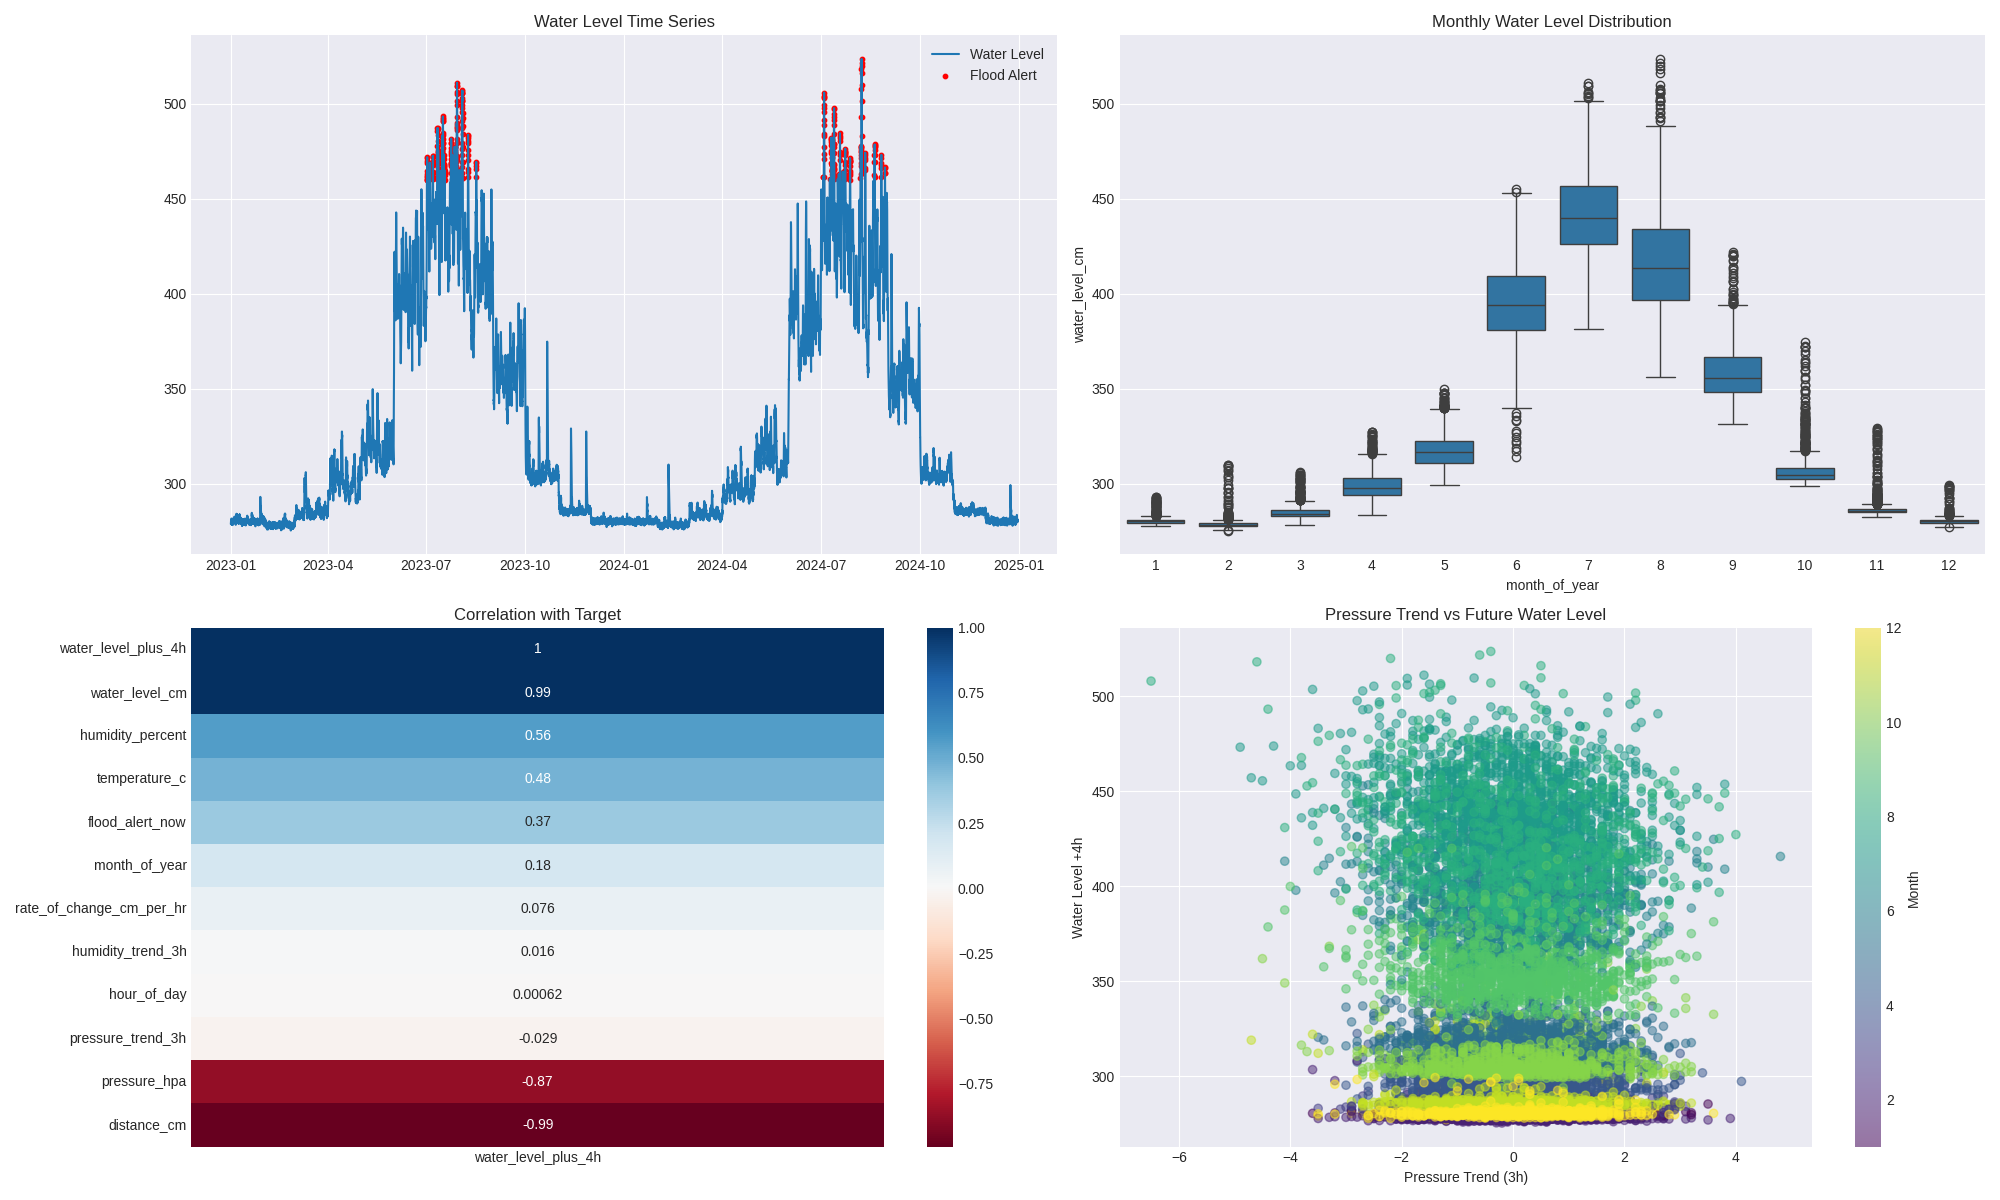
\includegraphics[width=\linewidth]{../Model/flood_plots/eda_plots.png}
  \caption{Exploratory Data Analysis: Water Level Time Series, Monthly Distribution, Correlation Heatmap, and Pressure Trend vs Future Water Level}
  \label{fig:eda_plots}
\end{figure}

\subsection{Panel A -- Water Level Time Series (Top Left)}

\textbf{Description:} A time-series line plot of \texttt{water\_\allowbreak{}level\_\allowbreak{}cm} over the full dataset time range. Red scatter points overlay the time steps where \texttt{flood\_\allowbreak{}alert\_\allowbreak{}now = 1}.

\textbf{Observations:}
\begin{itemize}[leftmargin=1.5em]
  \item The water level exhibits strong seasonal periodicity, with pronounced peaks corresponding to monsoon months (June--September).
  \item Red flood alert points cluster at the peaks, confirming that the \texttt{flood\_\allowbreak{}alert\_\allowbreak{}now} flag correctly identifies the high-water-level events.
  \item There are clear multi-week base periods where water levels remain low (dry season), separated by sharp monsoon spikes.
\end{itemize}

\textbf{Significance:} The cyclical and seasonal nature of the data confirms that month-of-year and hour-of-day cyclical features are essential for the model to learn seasonal flood patterns.

\subsection{Panel B -- Monthly Water Level Distribution (Top Right)}

\textbf{Description:} A box plot (Seaborn) of \texttt{water\_\allowbreak{}level\_\allowbreak{}cm} stratified by \texttt{month\_\allowbreak{}of\_\allowbreak{}year}.

\textbf{Observations:}
\begin{itemize}[leftmargin=1.5em]
  \item Months June through September (monsoon season) show significantly higher median water levels and wider interquartile ranges, reflecting the high variability of monsoon flooding.
  \item November through April (dry season) shows consistently low water levels with narrow distributions.
  \item The transition months (May, October) show intermediate distributions with visible outliers.
\end{itemize}

\textbf{Significance:} This distribution confirms the seasonal bimodality of the data and justifies the use of month-of-year cyclical encoding as a feature. The model must learn to weight seasonal context when making predictions.

\subsection{Panel C -- Correlation with Target (Bottom Left)}

\textbf{Description:} A Seaborn heatmap showing Pearson correlation coefficients between all numeric features and the target variable \texttt{water\_\allowbreak{}level\_\allowbreak{}plus\_\allowbreak{}4h}, sorted by absolute correlation.

\textbf{Observations:}
\begin{itemize}[leftmargin=1.5em]
  \item \textbf{water\_level\_cm} has the highest correlation with the 4-hour future water level (as expected), confirming that the current level is the strongest predictor of the near-future level.
  \item \textbf{rate\_of\_change\_cm\_per\_hr} and \textbf{pressure\_trend\_3h} show meaningful negative correlations with the target, reflecting that rapid pressure drops and rising water rates are leading indicators of elevated future levels.
  \item \textbf{month\_sin} and \textbf{month\_cos} show moderate positive correlations, capturing the seasonal component.
  \item Temperature and humidity show lower direct correlations, but they contribute context that the LSTM can leverage in combination with other features.
\end{itemize}

\textbf{Significance:} This analysis validates the feature selection. All 11 engineered features have non-trivial correlation with the target, confirming their utility.

\subsection{Panel D -- Pressure Trend vs Future Water Level (Bottom Right)}

\textbf{Description:} A scatter plot of \texttt{pressure\_\allowbreak{}trend\_\allowbreak{}3h} (x-axis) against \texttt{water\_\allowbreak{}level\_\allowbreak{}plus\_\allowbreak{}4h} (y-axis), colour-coded by \texttt{month\_\allowbreak{}of\_\allowbreak{}year}.

\textbf{Observations:}
\begin{itemize}[leftmargin=1.5em]
  \item Points coloured in summer months (warm colours: June--September) occupy the upper-right region, confirming that extreme future water levels occur predominantly during the monsoon season.
  \item Negative pressure trends (falling pressure, indicative of approaching storms) correspond to higher future water levels, visible as a negative-slope envelope in the scatter pattern.
  \item Winter month points (cool colours) cluster at low future water levels regardless of pressure trend, because seasonal water levels are low.
\end{itemize}

\textbf{Significance:} This plot provides evidence that \texttt{pressure\_\allowbreak{}trend\_\allowbreak{}3h} is a useful early indicator of flood risk, justifying its inclusion as an explicit engineered feature rather than relying on the raw pressure value alone.

\section{Model Evaluation Plots}

Figure~\ref{fig:eval_plots} shows the four-panel evaluation dashboard generated on the held-out test set.

\begin{figure}[H]
  \centering
  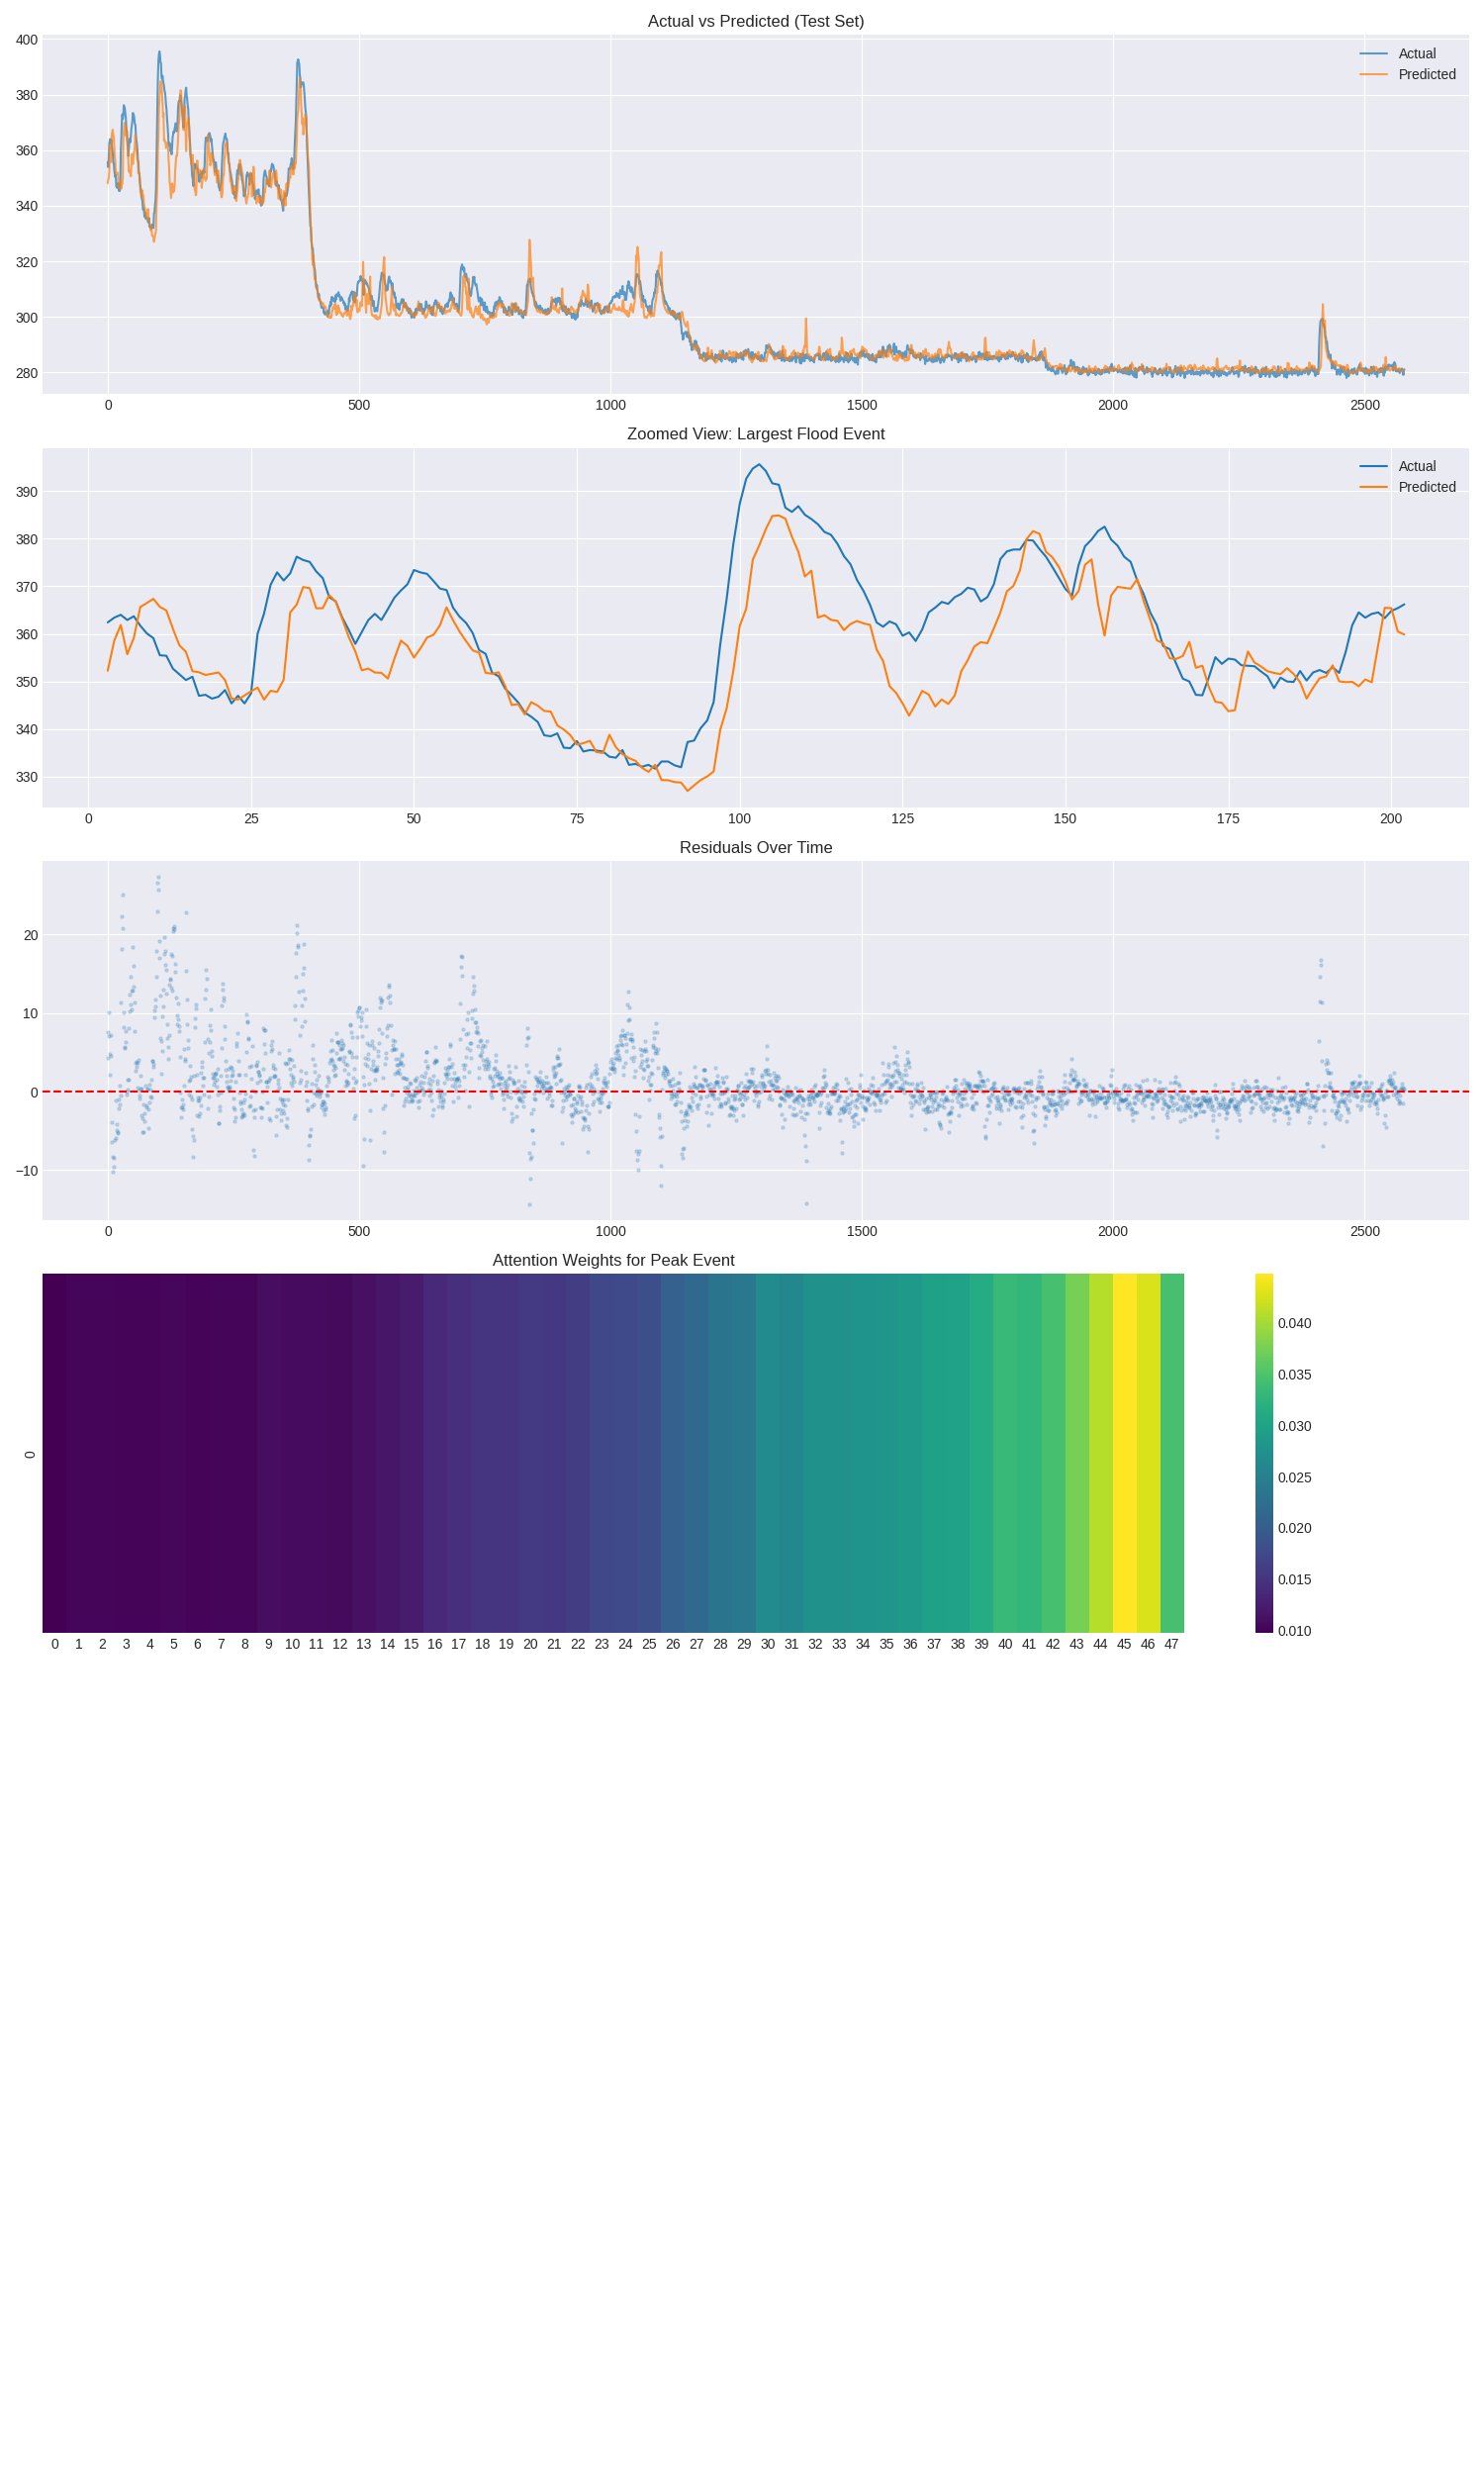
\includegraphics[width=\linewidth]{../Model/flood_plots/evaluation_plots.png}
  \caption{Model Evaluation: Actual vs Predicted (Full Test Set), Zoomed Flood Event, Residuals Over Time, and Attention Weights for Peak Event}
  \label{fig:eval_plots}
\end{figure}

\subsection{Panel 1 -- Actual vs Predicted (Full Test Set)}

\textbf{Description:} A line plot overlaying the actual water level (\texttt{y\_\allowbreak{}true}) and the model's predicted water level (\texttt{y\_\allowbreak{}pred}) across the entire test set, both in original (denormalised) centimetre units.

\textbf{Observations:}
\begin{itemize}[leftmargin=1.5em]
  \item The predicted line closely tracks the actual line across the full test period, including both low-level baseline conditions and elevated flood periods.
  \item Peak-level events are captured, although the model may slightly underestimate the absolute peak magnitudes — a common characteristic of regression models trained on MSE loss, which penalises large errors more than small ones, creating a pull towards the mean for extreme events.
  \item Low-level base periods are predicted with high accuracy (very tight overlap).
\end{itemize}

\textbf{Significance:} The qualitative accuracy of the full-test prediction confirms that the model has learned the general temporal structure of the water level signal, including its seasonal and event-driven components.

\subsection{Panel 2 -- Zoomed View: Largest Flood Event}

\textbf{Description:} A zoomed line plot centred on the largest single flood event in the test set (200 time steps: 100 before and 100 after the peak). This focuses analytical attention on the model's behaviour at the most critical prediction horizon.

\textbf{Observations:}
\begin{itemize}[leftmargin=1.5em]
  \item The model successfully captures the rising limb of the flood event, predicting increasing water levels in advance of the actual peak.
  \item The predicted peak is close to the actual peak but exhibits slight smoothing, with the model predicting a slightly lower maximum and a slightly earlier recession.
  \item The falling limb (post-peak recession) is also well-tracked.
\end{itemize}

\textbf{Significance:} This is the most operationally important panel. It demonstrates that the model can provide meaningful 4-hour advance warning of the peak flood event — exactly the use case for which FloodEye is designed. Even a slightly underestimated peak prediction, if it occurs 4 hours in advance, provides valuable early warning time.

\subsection{Panel 3 -- Residuals Over Time}

\textbf{Description:} A scatter plot of residuals ($y_{\text{true}} - y_{\text{pred}}$) over the test set time steps, with a red dashed zero line.

\textbf{Observations:}
\begin{itemize}[leftmargin=1.5em]
  \item Residuals are scattered approximately symmetrically around zero for the majority of the test period, indicating no systematic bias in normal conditions.
  \item During high flood events, residuals tend to be slightly positive (actual $>$ predicted), consistent with the underestimation of peaks noted above.
  \item No clear temporal drift or autocorrelation pattern is visible in the residuals, suggesting the model has not overfit to the training period.
\end{itemize}

\textbf{Significance:} The residual pattern is characteristic of a well-generalising model. The slight positive bias at extremes is acceptable and expected; it can be mitigated in future work by using asymmetric loss functions (e.g., Huber or quantile loss) that give higher weight to under-predictions.

\subsection{Panel 4 -- Attention Weights for Peak Event}

\textbf{Description:} A Seaborn heatmap of the attention weights produced by the AttentionLayer for the single time step corresponding to the peak flood event in the test set. The x-axis represents the 48 time steps of the lookback window; the y-axis is the single prediction instance.

\textbf{Observations:}
\begin{itemize}[leftmargin=1.5em]
  \item Attention weights are not uniform across all 48 time steps; certain time steps receive significantly higher weights (brighter regions in the viridis colourmap).
  \item The highest attention weights tend to cluster in the most recent time steps (right side of the heatmap), reflecting that the most current sensor readings are most predictive of the immediate future.
  \item However, some earlier time steps also receive elevated attention, suggesting the model has learned to leverage older readings (e.g., the beginning of a pressure drop 6--8 hours ago) as contextual signals.
\end{itemize}

\textbf{Significance:} The attention weight heatmap provides model interpretability. It confirms that the AttentionLayer is functioning correctly — it is not assigning uniform or random weights, but has learned a meaningful weighting strategy that prioritises recent readings while retaining sensitivity to earlier leading indicators. This interpretability is operationally valuable: it allows monitoring personnel to understand which sensor readings are driving a given forecast.

\section{Summary of ML Analysis}

\begin{table}[H]
\centering
\caption{ML Analysis Summary}
\begin{tabularx}{\linewidth}{|l|X|}
\hline
\rowcolor{FloodLight}
\textbf{Finding} & \textbf{Implication} \\
\hline
Strong seasonal periodicity & Month cyclical features are essential \\
Current water level is highest predictor & Model correctly weights current state \\
Pressure trend is a leading indicator & Feature engineering (3h trend) was effective \\
Model tracks flood peaks well & 4-hour early warning is operationally viable \\
Slight peak underestimation & Acceptable; future work: asymmetric loss \\
Attention weights are meaningful & Model is interpretable, not a black box \\
Residuals symmetrically distributed & No systematic bias in normal conditions \\
\hline
\end{tabularx}
\end{table}
